\section{Introducción}

\subsection{1.1 Motivación y Contexto}

Resulta revelador observar cómo la percepción remota ha evolucionado de capturas aisladas a sistemas capaces de integrar múltiples dimensiones de la realidad terrestre. En aplicaciones críticas como el monitoreo de desastres naturales, la gestión agrícola de precisión y la vigilancia ambiental, contar con información completa y oportuna marca la diferencia entre anticipar un evento o simplemente documentar sus consecuencias. Los sensores hiperespectrales (HSI) entregan firmas espectrales ricas que permiten distinguir materiales y estados bioquímicos con gran detalle, mientras que el radar de apertura sintética (SAR) ofrece robustez frente a condiciones atmosféricas adversas, penetración parcial y sensibilidad a estructuras y humedad.

Esta complementariedad no es nueva, pero su explotación sistemática ha ganado impulso decisivo con el avance de las redes neuronales profundas. \cite{Li2022Deep} destacan en su revisión exhaustiva cómo los enfoques basados en aprendizaje profundo han transformado la fusión multimodal en teledetección, logrando mejoras sustanciales en precisión y robustez que los métodos tradicionales rara vez alcanzaban. Particularmente llamativo es el potencial que surge cuando se combinan las cientos de bandas estrechas del HSI con la información geométrica y dieléctrica del SAR: el resultado tiende a superar las limitaciones individuales de cada modalidad, especialmente en escenarios donde la nubosidad, la oscuridad o la complejidad del terreno reducen drásticamente la utilidad de observaciones ópticas aisladas.

\begin{table*}[h]
\centering
\caption{Comparativa de características principales entre sensores hiperespectrales y SAR}
\label{tab:comparativa_sensores}
\begin{tabular}{lcc}
\hline
\textbf{Característica} & \textbf{HSI} & \textbf{SAR} \\
\hline
Resolución espectral & Muy alta (cientos de bandas) & Baja (bandas polarimétricas) \\
Penetración atmosférica & Limitada (afectada por nubes) & Alta \\
Sensibilidad a estructura & Baja & Alta \\
Información material & Muy alta & Media (diélectrica) \\
Disponibilidad temporal & Dependiente de iluminación & Día/noche, todo clima \\
\hline
\end{tabular}
\end{table*}

\begin{figure}[h]
\centering
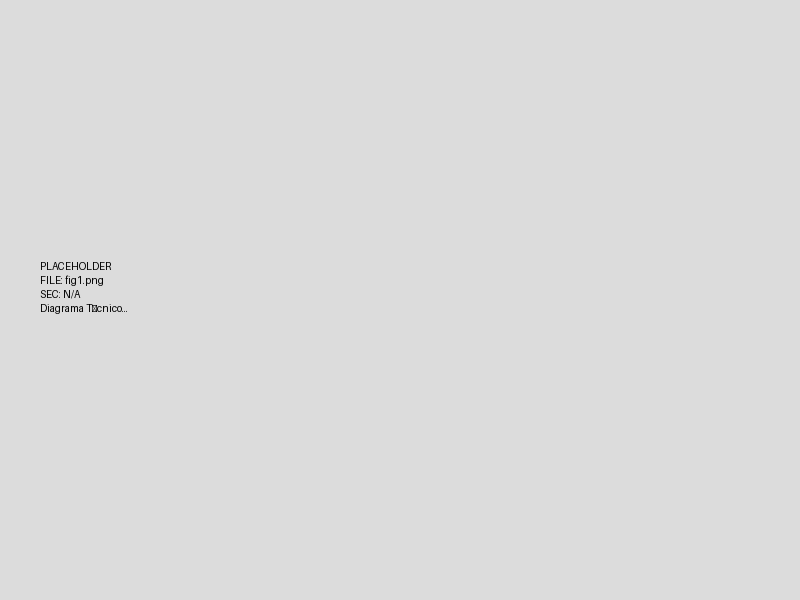
\includegraphics[width=\linewidth]{fig1.png}
\caption{Esquema conceptual de la integración multimodal HSI-SAR mediante fusión profunda para monitoreo crítico.}
\label{fig:esquema_conceptual}
\end{figure}

\subsection{1.2 Desafíos en Fusión Multimodal}

Uno de los desafíos persistentes que surge al analizar estos sistemas radica en la heterogeneidad fundamental de las modalidades. Las diferencias en resolución espacial, alineación geométrica, naturaleza del ruido y representaciones de características complican enormemente el proceso de fusión. En muchos casos estudiados, los métodos tempranos basados en reglas o transformaciones lineales mostraron mejoras modestas, pero tendían a fallar ante variabilidad real del terreno o condiciones operativas extremas.

Aunque los enfoques de aprendizaje profundo han mitigado varios de estos problemas, no los han eliminado. \cite{Li2022Deep} subrayan que la brecha entre la riqueza espectral y la robustez estructural sigue requiriendo arquitecturas sofisticadas capaces de modelar interacciones cruzadas de forma efectiva. A esto se suma la complejidad computacional, el riesgo de sobreajuste en datasets limitados y la necesidad de interpretabilidad en aplicaciones donde las decisiones impactan directamente en seguridad o políticas públicas.

Hong y colaboradores, en su panorama general de la fusión multimodal, ilustran claramente la transición desde métodos superficiales hacia enfoques profundos, destacando brechas aún abiertas en escenarios de monitoreo crítico donde la latencia y la confiabilidad resultan críticas \cite{Hong2021Overview}.

\subsection{1.3 Contribuciones}

Lejos de ser un asunto resuelto, este trabajo busca contribuir de manera concreta a cerrar algunas de esas brechas. La presente investigación propone una arquitectura de fusión asimétrica basada en redes neuronales profundas que integra mecanismos de atención cruzada multi-escala, aprovechando las fortalezas espectrales del HSI y las propiedades estructurales del SAR de forma más equilibrada que enfoques previos.

Entre las contribuciones principales destacan: (i) el diseño de un módulo de extracción y fusión multimodal adaptado específicamente a la heterogeneidad HSI-SAR, (ii) una evaluación exhaustiva en conjuntos de datos públicos representativos de escenarios reales, y (iii) un análisis crítico de robustez bajo condiciones adversas que suele omitirse en la literatura. 

De esta manera, las siguientes secciones revisan el estado del arte, detallan la metodología propuesta, presentan los resultados experimentales y discuten implicaciones prácticas junto con direcciones futuras.